 % ****** Start of file apssamp.tex ******
%
%   This file is part of the APS files in the REVTeX 4.2 distribution.
%   Version 4.2a of REVTeX, December 2014
%
%   Copyright (c) 2014 The American Physical Society.
%
%   See the REVTeX 4 README file for restrictions and more information.
%
% TeX'ing this file requires that you have AMS-LaTeX 2.0 installed
% as well as the rest of the prerequisites for REVTeX 4.2
%
% See the REVTeX 4 README file
% It also requires running BibTeX. The commands are as follows:
%
%  1)  latex apssamp.tex
%  2)  bibtex apssamp
%  3)  latex apssamp.tex
%  4)  latex apssamp.tex

\documentclass[%
reprint,
%superscriptaddress,
%groupedaddress,
%unsortedaddress,
%runinaddress,
%frontmatterverbose, 
%preprint,
%preprintnumbers,
twocolumn,
nofootinbib,
%nobibnotes,
%bibnotes,
 amsmath,amssymb,
 aps,
%pra,
%prb,
%rmp,
%prstab,
%prstper,
%floatfix,
]{revtex4-2}
\usepackage{siunitx}
\usepackage{physics}
\usepackage{braket}
\usepackage{graphicx}
\usepackage{subcaption}
\usepackage[caption=false]{subfig}
% Include figure files
\usepackage{dcolumn}% Align table columns on decimal point
\usepackage{bm}% bold math
%\usepackage{hyperref}% add hypertext capabilities
%\usepackage[mathlines]{lineno}% Enable numbering of text and display math
%\linenumbers\relax % Commence numbering lines
\usepackage{float}
%\usepackage[showframe,%Uncomment any one of the following lines to test 
%%scale=0.7, marginratio={1:1, 2:3}, ignoreall,% default settings
%%text={7in,10in},centering,
%%margin=1.5in,
%%total={6.5in,8.75in}, top=1.2in, left=0.9in, includefoot,
%%height=10in,a5paper,hmargin={3cm,0.8in},
%]{geometry}
\usepackage{xcolor}
\usepackage[symbol,hang,flushmargin]{footmisc}

\usepackage{graphicx} % Required for inserting images
\usepackage{amsmath}
\usepackage{amssymb}
\usepackage{subcaption}
\usepackage{etoolbox,lipsum}

\begin{document}

\preprint{APS/123-QED}

\title{
%\includegraphics[width=0.7\textwidth]{img/teaser.png}\\
%Bean There, Done That: A Mathematical Model of Bean Sculptures
Bean There, Done That: Computer-Assisted Design of Bean Sculptures}

\author{Dave Pagurek$^{1,*}$}
%\email{Milica.Banic@nrc-cnrc.gc.ca} 
\footnotetext[1]{davepagurek@gmail.com}
\author{Milica Banic$^2$}
\affiliation{$^1$ Bean Futurists Society\\$^2$Institute for Advanced Legume Research, Bohnestrasse 3000, Munich, Germany}

\date{\today}% It is always \today, today,
             %  but any date may be explicitly specified

\begin{abstract}
Chicago's status as a world-class city is cemented by its iconic bean sculpture. Other cities, wanting to replicate the success, have muddied the bean waters by introducing their own bean variations: New York City has a bean sharing similar properties, and Ottawa has a sphere, dubbed the ``Ottawa bean'' by locals. Our economic analysis proves their worth, so naturally other cities will want their own. We present a mathematical model of the space of all bean sculptures, and an algorithm to help cities replace existing landmarks with beans.
\end{abstract}

%\keywords{Suggested keywords}%Use showkeys class option if keyword
                              %display desired
\maketitle
%\tableofcontents

\onecolumngrid

\begin{figure}[h]
    \centering
    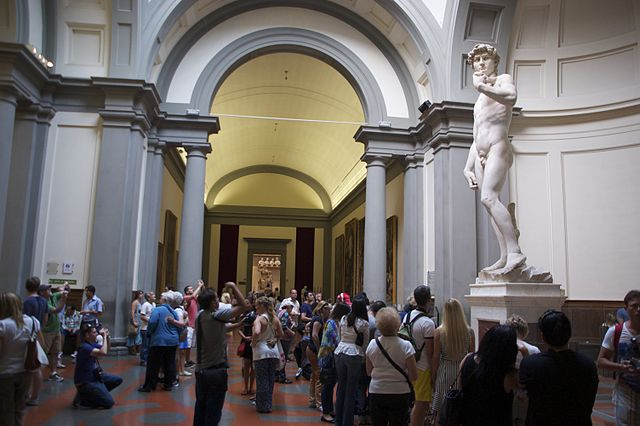
\includegraphics[width=0.44\linewidth]{img/david-tourists.jpg}
        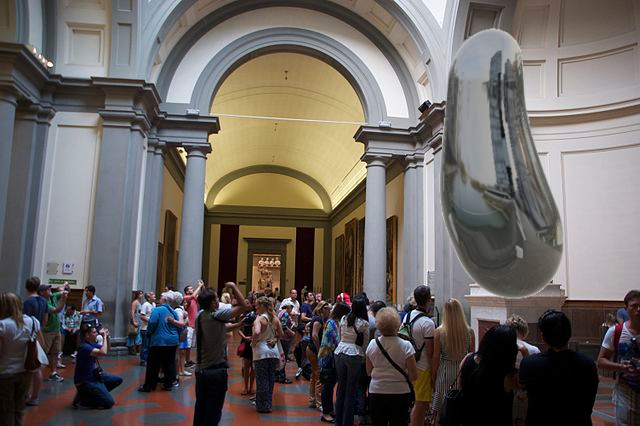
\includegraphics[width=0.44\linewidth]{img/david-tourists-bean.jpg}
    \caption{Michaelangelo's \emph{David} improved by being turned into a bean sculpture (photo by Wikimedia Commons Korido, CC BY-SA 4.0)}
    \label{fig:teaser}
\end{figure}
\twocolumngrid

\section{Introduction}

Public art is important: It can serve as an expression of culture, heritage, and creativity within a community. It has the power to stimulate dialogue and provoke thought. It is a nice thing to go look at with one's friends\footnotemark[4]\footnotetext[4]{This is true even if one's friends misrepresent the nature of the public art to which one is being led.}, or to walk past on one's way to work. On top of this, successful public art installations can contribute to the economic vitality of a city by attracting tourists, fostering a sense of place, and enhancing the overall appeal of urban environments. Indeed, successful public art can become an icon for its host city, putting it on the map in a way that is not otherwise possible. 

Consider as an example ``The Bean" (known to nerds and um ackchuyually types as ``Cloud Gate"), a sculpture by artist Anish Kapoor that was unveiled in Chicago in 2006~\cite{City}. Almost 20 years after its construction, the Bean stands as a symbol of Chicago and a success story of public art. Having observed the Bean's impact (perhaps even feeling threatened by it) New York City, a city with no dearth of art and culture, commissioned another bean structure from Kapoor, which was completed in 2023. Naturally one begins to suspect that we are seeing the beginnings of a revolution within the art world and public life more broadly.

As the saying goes, twice is a coincidence, but three times is a pattern: Recently, a bean-like structure has been rediscovered by locals in Ottawa, Ontario. The piece was built in 1966 and originally called ``The Sphere"~\cite{Waymarking}, but it has recently enjoyed a surge in popularity since its rebranding as ``The Ottawa Bean". Though less curvy than Chicago's, Ottawa bean is still a bean. In fact, it is the simplest bean (that is, the trivial bean), the result of taking away all possible bends and dimples.

The growing success of this third reflective bean cements the potential of bean structures to revolutionize public art. It is important to note that the Ottawa Bean is not by any particularly famous artist\footnotemark[2]\footnotetext[2]{The authors mean no offense to Art Price, progenitor of the Ottawa Bean, but he does not have a Wikipedia page and that's just a fact.}. This point solidifies the intuition that the reflectivity and bean morphology are the key factors in the beans' appeal, rather than some arcane feature of Anish Kapoor's style in particular. This begs the question: How far can we take this? Can other communities emulate the success of these three beans? And how can one create a bean for one's own city?

One possibility would be to commission artists, but communities may be deterred from this option due to artists' sometimes difficult personalities, and their insistence on being paid for their work. A more pragmatic option would be to automate the design of the beans; this is a realistic possibility, due to the beans' simple forms. Although one could randomize the bean parameters, this kind of approach could be criticized for not actually being art, due to a lack of inspiration or underlying meaning. We propose an approach in which beans are designed based on other objects; in particular, here we base our designs off iconic landmarks, with the intention of eventually replacing them with beans to maximize the impact of the new beans.

In Section \ref{section:background} we present some general background to motivate the construction of more bean sculptures. In Section \ref{sec:method} we outline a mathematical model for beans that can neatly describe existing beans, but is flexible enough to accommodate a variety of new beans in a similar style. We accomplish this by formulating beans as a signed distance function for the smooth union of one or more quadratic B\'ezier curves. The existing and agreed-upon bean sculptures fit nicely into the parameter space (``bean-space'') as single curves, while compound beans can reproduce structures visually similar to other city landmarks while still appearing definitively like a bean. To help along the bean-hopeful, in Section \ref{section:bestfit} we provide an algorithm to automatically fit existing city structures into their nearest bean-space equivalent. In Section \ref{section:results} we apply the model to some examples, and we conclude in Section \ref{section:conclusion}.


%\textcolor{red}{((old intro))}

%Cities around the world have started to fill their public spaces with large, reflective bean sculptures, shown in Figure~\ref{fig:sculptures}. People flock to the beans in droves, putting their host cities on the map in a way a beanless city never could. As the beans proliferate and more cities erect their own unique takes on the bean theme, one is left to wonder, what drives this bean craze? What can beans do for your city? What does it mean to be a bean? And how can one create a bean for one's own city?

%We provide much-needed answers to these questions. We crunch the numbers on existing beans to figure out why they're important. Then, we describe a mathematical model for beans that can neatly describe existing beans but is flexible enough to accommodate a variety of new beans in a similar style. 

%We accomplish this by formulating beans as a signed distance function for the smooth union of one or more quadratic B\'ezier curves. The existing and agreed-upon bean sculptures fit nicely into the parameter space (``bean-space'') as single curves, while compound beans can reproduce structures visually similar to other city landmarks while still appearing definitively like a bean. To help along the bean-hopeful, we provide an algorithm to automatically fit existing city structures into their nearest bean-space equivalent.

\begin{figure}
    \begin{subfigure}{0.15\textwidth}
        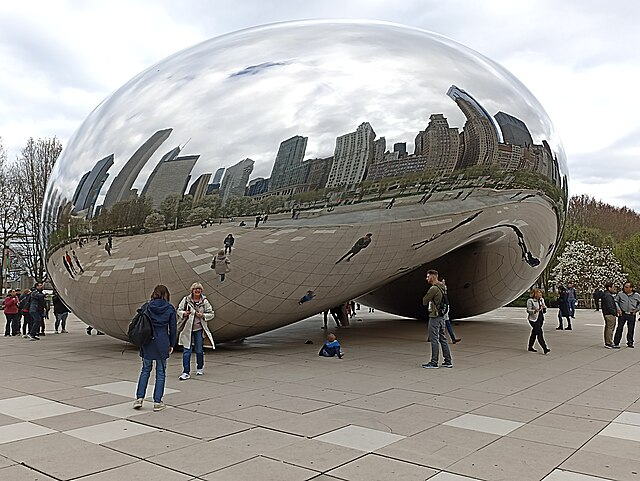
\includegraphics[width=0.98\linewidth]{img/Cloud_Gate_1.jpg}
    \end{subfigure}
    \begin{subfigure}{0.15\textwidth}
        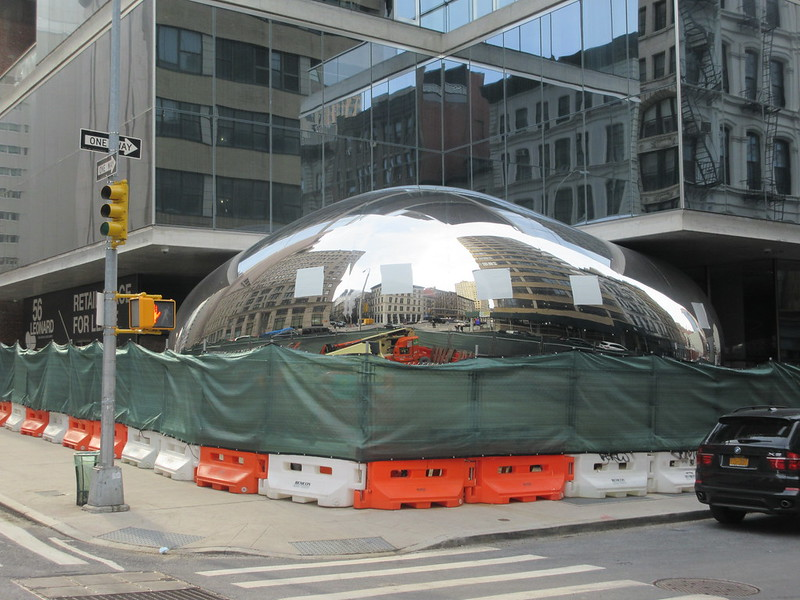
\includegraphics[width=0.98\linewidth]{img/nyc.jpg}
    \end{subfigure}
    \begin{subfigure}{0.15\textwidth}
        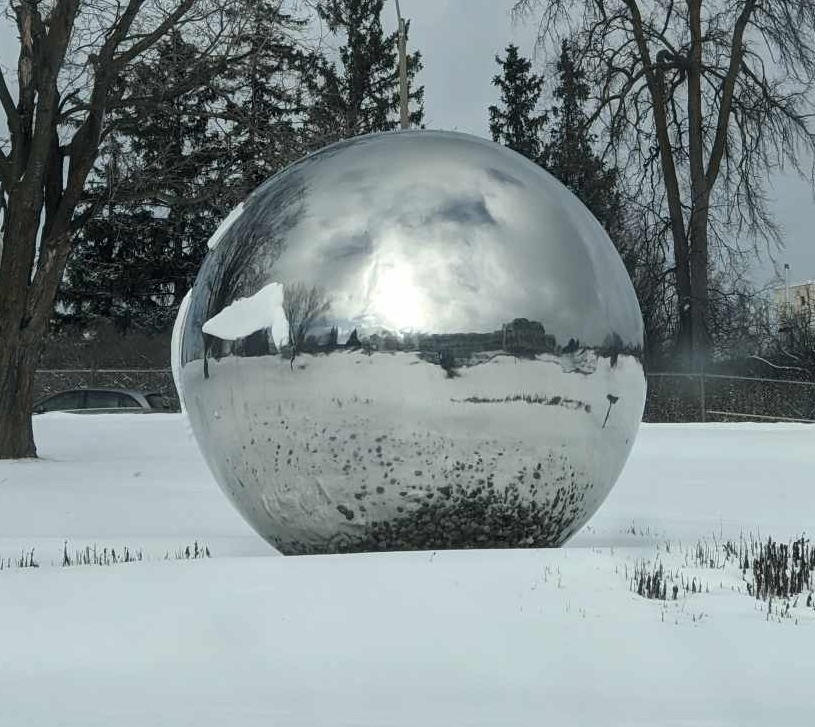
\includegraphics[trim={2.5cm 4cm 2.5cm 3.5cm},clip,width=0.98\linewidth]{img/ottawa-sphere.jpg}
    \end{subfigure}
    \caption{Beans in Chicago, New York City, and Ottawa, respectively. NYC photo \textcopyright Bracht Bug, CC BY-NC-ND 2.0.}
    \label{fig:sculptures}
\end{figure}


\section{Background}
\label{section:background}

%\subsection{Beans in the Wild}

%The most widely known bean sculpture, often referred to simply as ``The Bean'' (or ``Cloud Gate'' for nerds) was unveiled in Chicago in 2006.~\cite{City} The artist responsible, Anish Kapoor, was also commissioned to create a bean for the corner of a New York City skyscraper. Although less well known, Ottawa has had its own bean for longer: known to some as ``The Sphere'' and to others as ``Ottawa bean,'' artist Art Price erected a spherical bean in 1966.~\cite{Waymarking} Though less curvy than Chicago's, Ottawa bean is still a bean. In fact, it is the simplest bean, the result of taking away all possible bends and dimples.

\subsection{Why Beans?}

We begin with a brief economic argument for prioritizing the construction of bean sculptures. The first notable bean, the one in Chicago, provides ample reason for other cities to want to follow suit. It is situated in Millennium Park. Prior to construction of the bean, the park had a total of \emph{zero} annual visitors. After construction began, the city estimated it had 5 million annual visitors.~\cite{chicagoMayorEmanuel} That's an incalculable increase from 0. Figure~\ref{fig:ngram} shows how, in literature, references to Millennium Park went through the roof after construction of the bean began. In the first half of 2016, the city counted 12,859,360 visitors---approximately 26 million visitors annually---making it the ``\#1 attraction in the Midwest and among the top 10 most-visited sites in the U.S.''~\cite{chicagoMayorEmanuel}

That's a lot of visitors, but how does it stack up against other individual attractions? As a point of comparison, we look at Ottawa's Parliament Hill. In a 2007 report, it had just 3 million annual visitors.~\cite{ctvnewsParliamentHill} A recent restoration project for Parliament's Centre Block is budgeted as a \$4.5-5 billion project~\cite{canadaQuarterlyProgress}. Chicago's bean, meanwhile, costed just \$23 million.~\cite{theclareChicagoHistory}

We crunched the visitor numbers, and came to the following conclusion:
\begin{equation}
    \frac{\num[group-separator={,}]{5000000}}{\num[group-separator={,}]{3000000}} > 1
\end{equation}

We also crunched the numbers for the cost:
\begin{equation}
    \frac{\$\num[group-separator={,}]{23000000}}{\$\num[group-separator={,}]{4500000000}} < 1
\end{equation}

The natural conclusion that Ottawa would come to is that it would be more financially responsible to replace Parliament with a bean. As it is only a matter of time before other cities come to this conclusion, too, we provide an algorithm to replace something like Parliament with a bean for minimal disruption to the existing space.

\subsection{Why Replace Landmarks?}

We understand that cities may feel incentivized to simply build a new bean in a new location rather than replace existing landmarks. The main argument against this is an environmental one. A single bean will likely not satiate cities. If cities were to keep expanding every time they want a new bean, it would contribute to an unprecedented level of urban sprawl that is simply irresponsible in our present environmental crisis.

The other main reason to replace existing landmarks instead is because leaving landmarks in place impedes inevitable progress. We know that everything is chrome in the future~\cite{everythingChrome} and replacing landmarks with beans is a clear path to that future.

\begin{figure}
    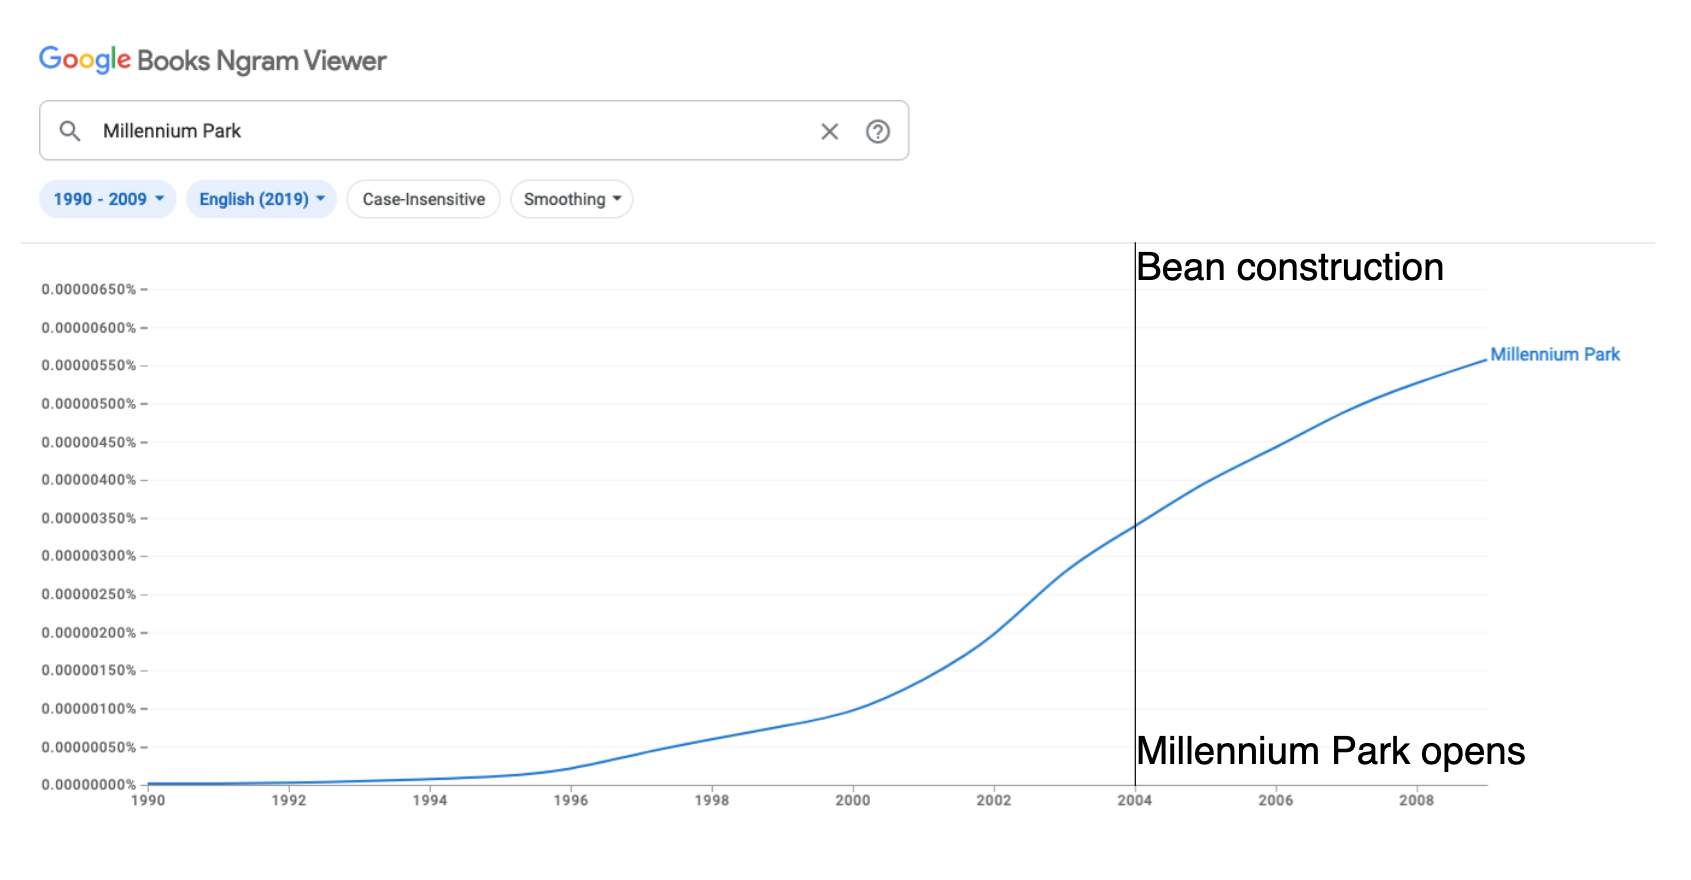
\includegraphics[width=0.98\linewidth]{img/ngram.png}
    \caption{Google Ngram Viewer data on references to Millennium Park in literature. Interest in Millennium Park skyrocketed in the leadup to and the introduction of the bean.}
    \label{fig:ngram}
\end{figure}

\section{Bean-Space Model}
\label{sec:method}

We use a quadratic B\'ezier as the base component of a bean since it is able to capture both the bent shape of the Chicago bean, but also in the trivial case where all control points are zero, the spherical Ottawa bean.

A single segment is unable to capture the potential range of all future beans, so we allow beans to be composed of multiple segments. Simply taking the union of multiple segments appears rigid and decidedly un-beanlike (see Figure~\ref{fig:smoothness}, left), so we instead define the surface in a way that allows us to use a \emph{smooth} union (see Figure~\ref{fig:smoothness}, right.) Signed Distance Functions allow such a smooth union to be defined succinctly, so we chose this format to represent our bean surfaces. This means that we represent the surface of a bean as the isosurface $f(X) = 0$, where $f$ describes the signed distance to the surface. At a high level, $f$ describes the smooth union between multiple quadratic B\'ezier segments.

\subsection{Signed Distance Functions}

A signed distance function (SDF) is a function $f: \mathbb{R}^n \mapsto \mathbb{R}$ describing the distance to a surface at a given point in space. Mapping out the isosurface of $f(X) = 0$ yields the surface described by the function. This can be done via the Marching Cubes algorithm to produce a 3D mesh, or via sphere tracing to produce an image.

SDFs are a flexible surface representation if one wants to organically join multiple base shapes. While taking $u(d_1,d_2)=\min\{d_1, d_2\}$ of two surfaces produces a surface representing the union of the shapes, the \emph{smooth union} operation $u(d_1,d_2)=d_1 + kg(d_2-d_1)/k)$ blends smoothly between its two inputs when they are a distance of $k$ apart, using the kernel $g$ to control the curve of the blending.

\subsection{Formulation}

Each quadratic B\'ezier segment is referenced in $f$ via a function representing the signed distance to the centerline of the segment, $Q(X; C)$.~\cite{iq2d} Here, $C \in R^{3 \times 3}$ describes the three control points to the function. For brevity, we omit the full definition of $Q$. We subtract a radius $r$ from $B$ to give the segment thickness.

In practice, we constrain $C$ such that $C_{i,1}=A_i$, $C_{i,3}=B_i$, and $C_{i,2} = (A_i + B_i)/2 + b\hat{n}$, where $b \in \mathbb{R}$ and $\hat{n}$ is a normalized vector such that $\hat{n} \dot (C_3 - C_1) = 0$. In effect, the middle control point is always halfway between the first and last control point, plus an offset normal to the line between them. This ensures a physically plausible curve with no self-intersections. Examples of segments fitting these constraints are shown in Figure~\ref{fig:bend}.

\begin{figure}
    \begin{subfigure}{0.1\textwidth}
        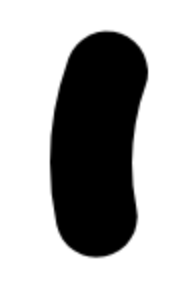
\includegraphics[width=0.98\linewidth]{img/seg5.png}
    \end{subfigure}
    \begin{subfigure}{0.2\textwidth}
        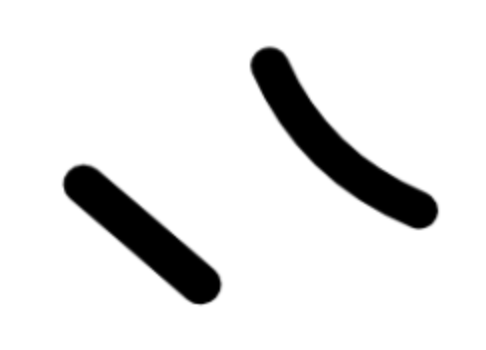
\includegraphics[width=0.98\linewidth]{img/seg3.png}
    \end{subfigure}
    \begin{subfigure}{0.15\textwidth}
        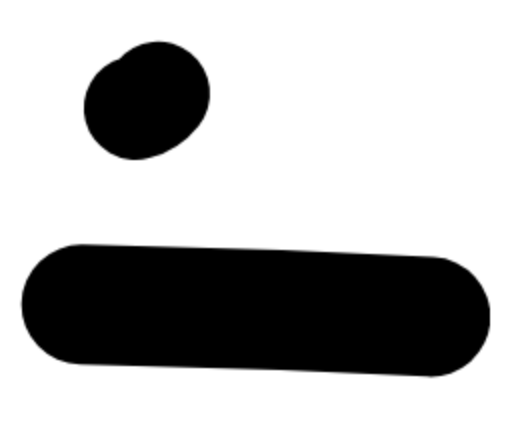
\includegraphics[width=0.98\linewidth]{img/seg4.png}
    \end{subfigure}
    \caption{Examples of different quadratic B\'ezier segments with our bend constraints.}
    \label{fig:bend}
\end{figure}

We combine each segment using the \emph{SDF smooth union operator} $U(d_1, d_2;k)$, which blends the distance between two input surface distances when they are a distance $k$ or less away:~\cite{iqsmooth}
\begin{equation}
    U(d_1, d_2; k) = d_1 + kg(d_2-d_1)/k
\end{equation}

Figure~\ref{fig:smoothness} shows the effect of the smoothness parameter $k$ on the final surface.

\begin{figure}
    \begin{subfigure}{0.15\textwidth}
        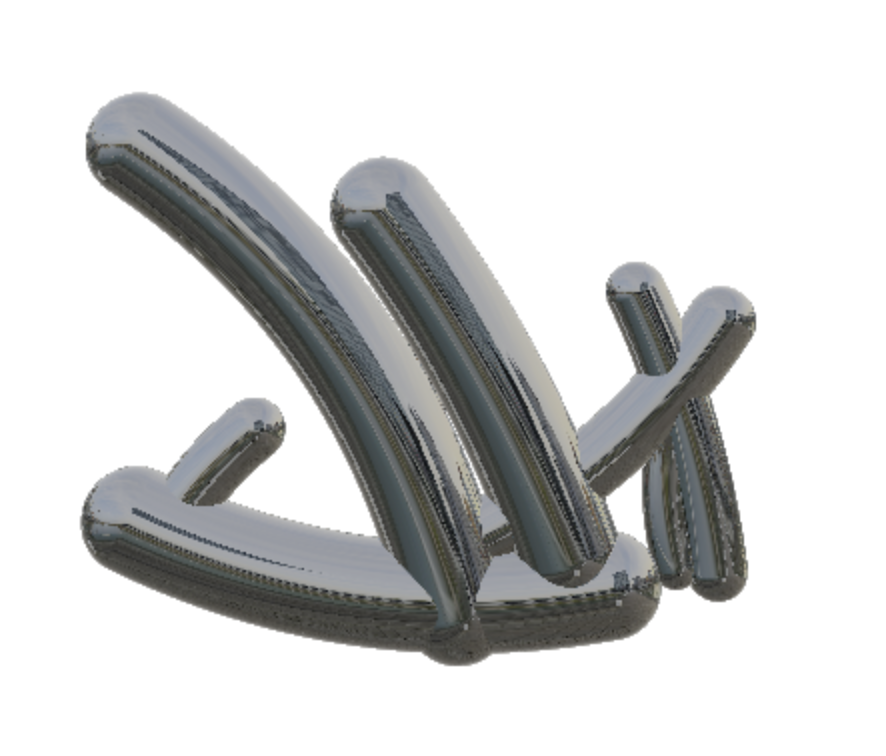
\includegraphics[width=0.98\linewidth]{img/smoothness0.png}
    \end{subfigure}
    \begin{subfigure}{0.15\textwidth}
        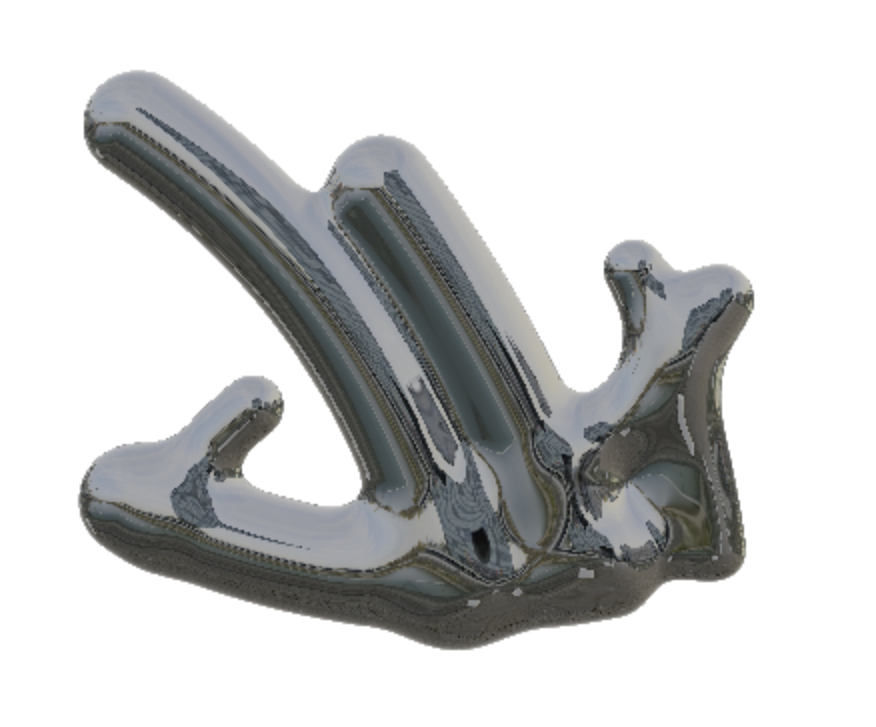
\includegraphics[width=0.98\linewidth]{img/smoothness0.05.png}
    \end{subfigure}
    \begin{subfigure}{0.15\textwidth}
        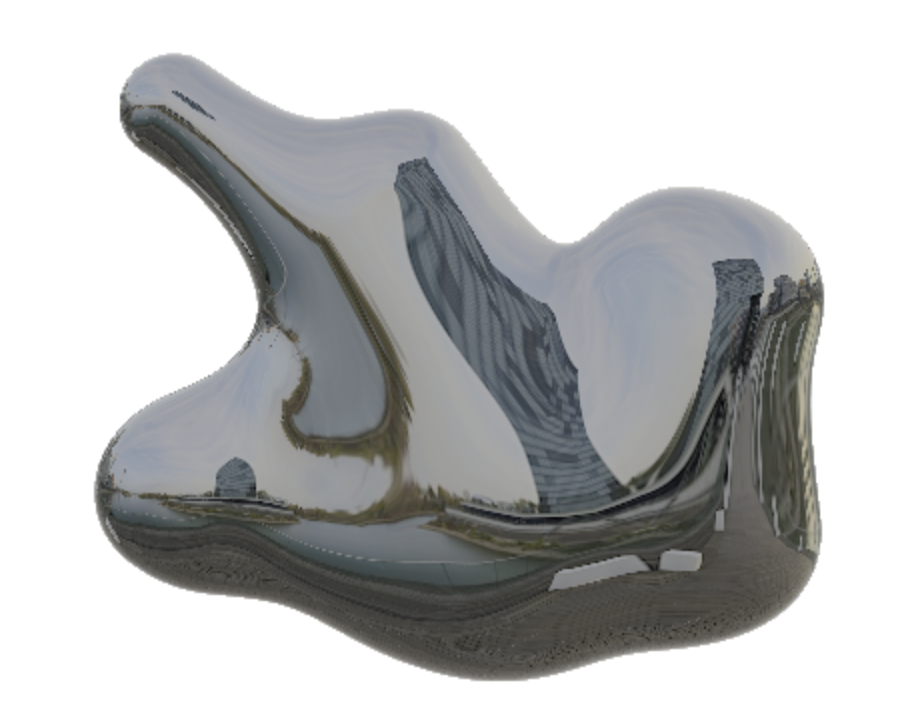
\includegraphics[width=0.98\linewidth]{img/smoothness0.2.png}
    \end{subfigure}
    \caption{Different values for the smoothness $k$ between segments: 0, 0.05, and 0.2, respectively.}
    \label{fig:smoothness}
\end{figure}

Using the above, we represent the bean surface $f$ recursively: the final value $f(X; n)$ is defined as the smooth union of the $n^\text{th}$ segment with $f(X; n-1)$, with the base case being a single segment:

\begin{equation}
    f(X; i) = \begin{cases}
        Q(X; C_0) - r_0, &i = 1\\
        U(B(X; C_i) - r_i, f(X; i-1), k), &i > 1\\
    \end{cases}
\end{equation}

To summarize, a bean in $f$ has the following parameters:

\begin{itemize}
    \item $n$, the number of B\'ezier segments
    \item $r_i$, $0 < i \le n$, the radius of each segment
    \item $A_i$, $0 < i \le n$, the start point for each segment
    \item $B_i$, $0 < i \le n$, the end point for each segment
    \item $b_i$, $0 < i \le n$, the amount of bend in each segment
    \item $k$, the smoothing between segments
\end{itemize}

\section{Bean of Best Fit}
\label{section:bestfit}


Given an target image, we want to optimize our bean-space parameters to find a bean that best matches the target. The target image $T$ is a $300 \times 300$-pixel one-bit image representing a mask of the space we want a bean to occupy. We define a function $P(n,r,A,B,b,k;T)$ that defines the score of a set of parameters in relation to the target image $T$. Using the bean-space parameters, we render similarly-sized image $M$ of the bean they represent. We then define $P$ as the intersection-over-union between the pixel grids $M$ and $T$. Maximizing this number encourages maximum coverage of the target area with minimal overlap with areas we don't want covered:

\begin{equation}
    P(M;T) = \frac{\sum_{i,j} M_{i,j} \land T_{i,j} }{\sum_{i,j} M_{i,j} \lor T_{i,j}}
\end{equation}

To perform the optimization, we need to use a method of optimization that does not rely exclusively on gradients, as the parameter $n$ is an integer and therefore does not have a useful gradient. We pick the Metropolis-Hastings algorithm to explore the space defined by our bean parameters as a probabilistic, gradient-free optimization algorithm.

\subsection{Metropolis-Hastings Optimization}

Markov Chain Monte Carlo (MCMC) algorithms are algorithms used to sample probability distributions $P(x)$ that are difficult to sample directly. In our case, bean-space, weighted by similarity to an input image, is such a difficult distribution.

The Metropolis-Hastings Algorithm is one such MCMC algorithm. Starting with one sample $x$ (in our case, a set of bean parameters), a new candidate sample $x'$ is selected from an easier-to-sample distribution, $Q(x' | x)$, such as by randomly mutating $x$. A random number $u \in [0,1]$ is generated: if $u < P(x')/P(x)$, the candidate sample is accepted; otherwise, it is rejected. Intuitively, a sample where $P(x)$ is higher than the current sample is always accepted, but there is still a chance of acceptance of lower-valued samples, too, allowing jumps into other areas of the distribution. This property is useful for exploring highly non-convex spaces.

To use this procedure for optimization, $P(x)$ can be treated as as function to optimize, and a record of the value of $x$ that produced the highest-seen value of $P(x)$ can be kept. This is effectively a zero-gradient optimization, since we only evaluate $P(x)$, not $dP(x)/dx$. This can be useful for mixed-integer optimization problems where a gradient would not exist. It also has the added benefit of being simple enough that the authors can implement it themselves, and not pay for an expensive license for optimization software.~\cite{gurobi}

\section{Results and Analysis}
\label{section:results}

% Pyramid image: https://en.wikipedia.org/wiki/Great_Pyramid_of_Giza#/media/File:Kheops-Pyramid.jpg
% Maman image: https://en.wikipedia.org/wiki/Maman_(sculpture)#/media/File:Giant_spider_strikes_again!.jpg

\subsection{Validation}

We found the  bean of best fit of known beans in order to validate the bean-fitting algorithm. The expected result would be a bean matching the shape of the input bean, as it is already a bean and does not need to be re-beaned. Both should only include one B\`ezier segment, and further, the Ottawa bean should have all its control points equal to 0 to form a sphere. Figure~\ref{fig:validation} shows the result of the optimization process when run on the Chicago and Ottawa beans, where it successfully matches the shape of the input.

\begin{figure}[h]
    \begin{subfigure}{0.23\textwidth}
        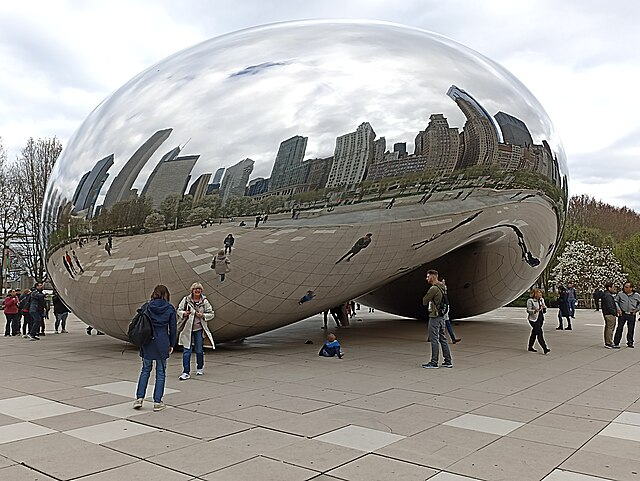
\includegraphics[width=0.98\linewidth]{img/Cloud_Gate_1.jpg}
    \end{subfigure}
    \begin{subfigure}{0.23\textwidth}
        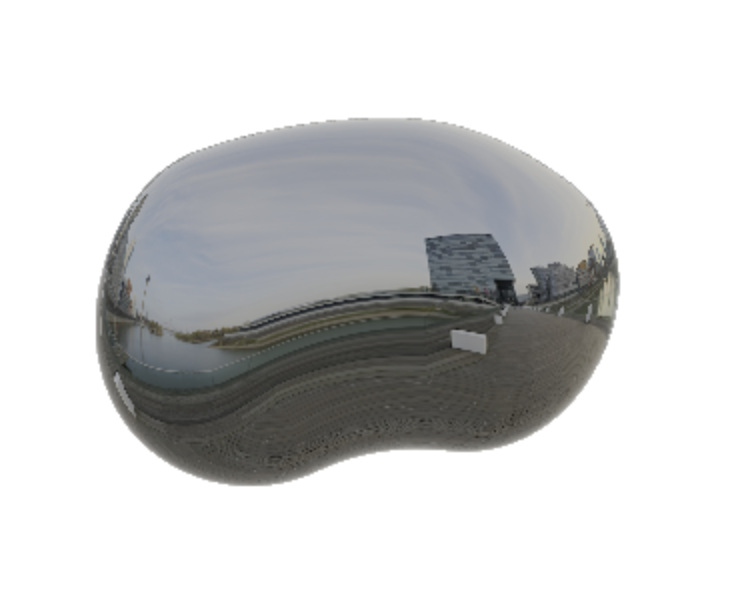
\includegraphics[width=0.98\linewidth]{img/bean-bean.png}
    \end{subfigure}
    \begin{subfigure}{0.23\textwidth}
        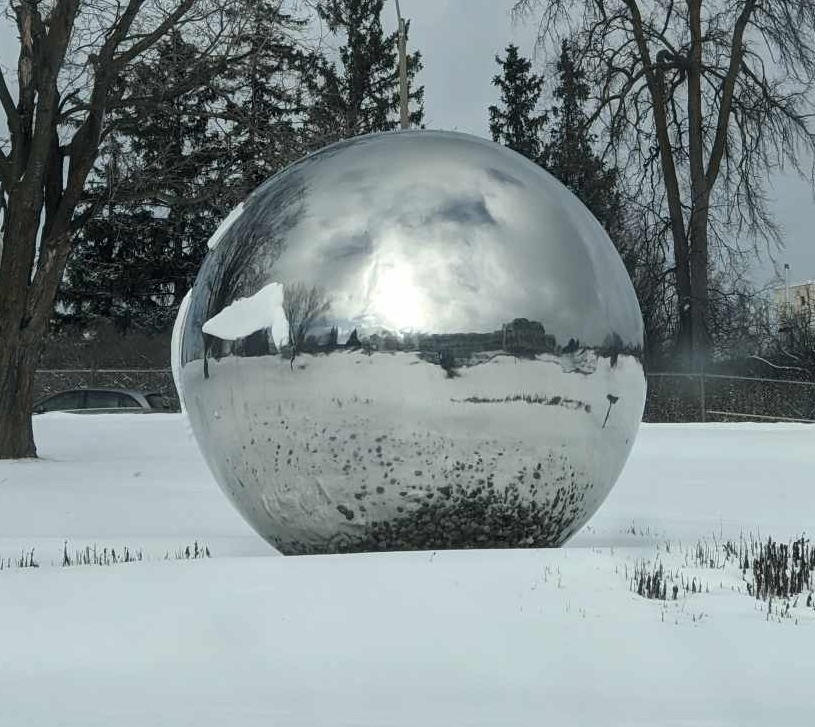
\includegraphics[width=0.98\linewidth]{img/ottawa-sphere.jpg}
    \end{subfigure}
    \begin{subfigure}{0.23\textwidth}
        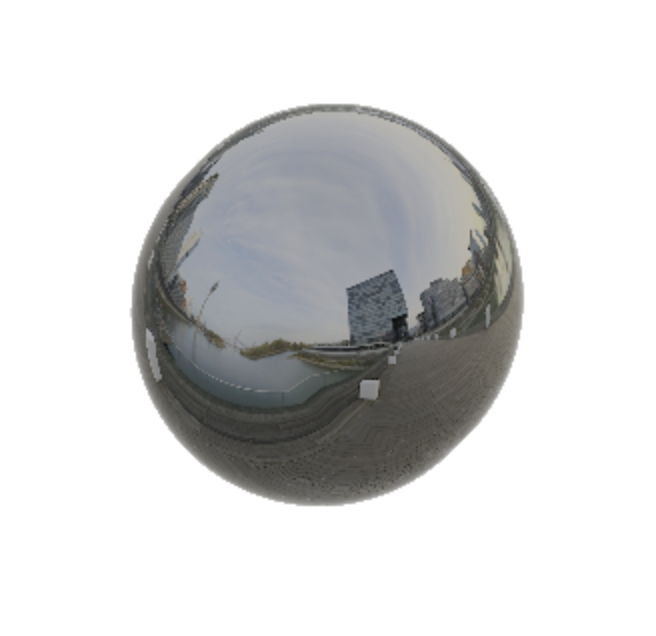
\includegraphics[width=0.98\linewidth]{img/sphere-bean.png}
    \end{subfigure}
    \caption{Existing beans recreated via our bean-fitting algorithm: Chicago's bean (top) and Ottawa's bean (bottom).}
    \label{fig:validation}
\end{figure}

Now that we know our bean-fitting algorithm works on existing beans, we explore its impact on replacing structures yet to be beaned.

Since the purpose of beaning a city is to place it on the map, it is natural that cities would want to ensure its bean is in a significant, easy-to-access location. A logical place to start, then, would be to replace a city's most notable landmarks with an equivalent bean. Figure~\ref{fig:ottawa} shows some examples of notable Ottawa landmarks: the Parliament buildings are maybe the motivation for most grade school field trips to Ottawa, but are unlikely to be a stand-out attraction in the eyes of the students visiting. A bean replacement will increase tourist satisfaction with no downsides.

\begin{figure}[H]
    \begin{subfigure}{0.23\textwidth}
        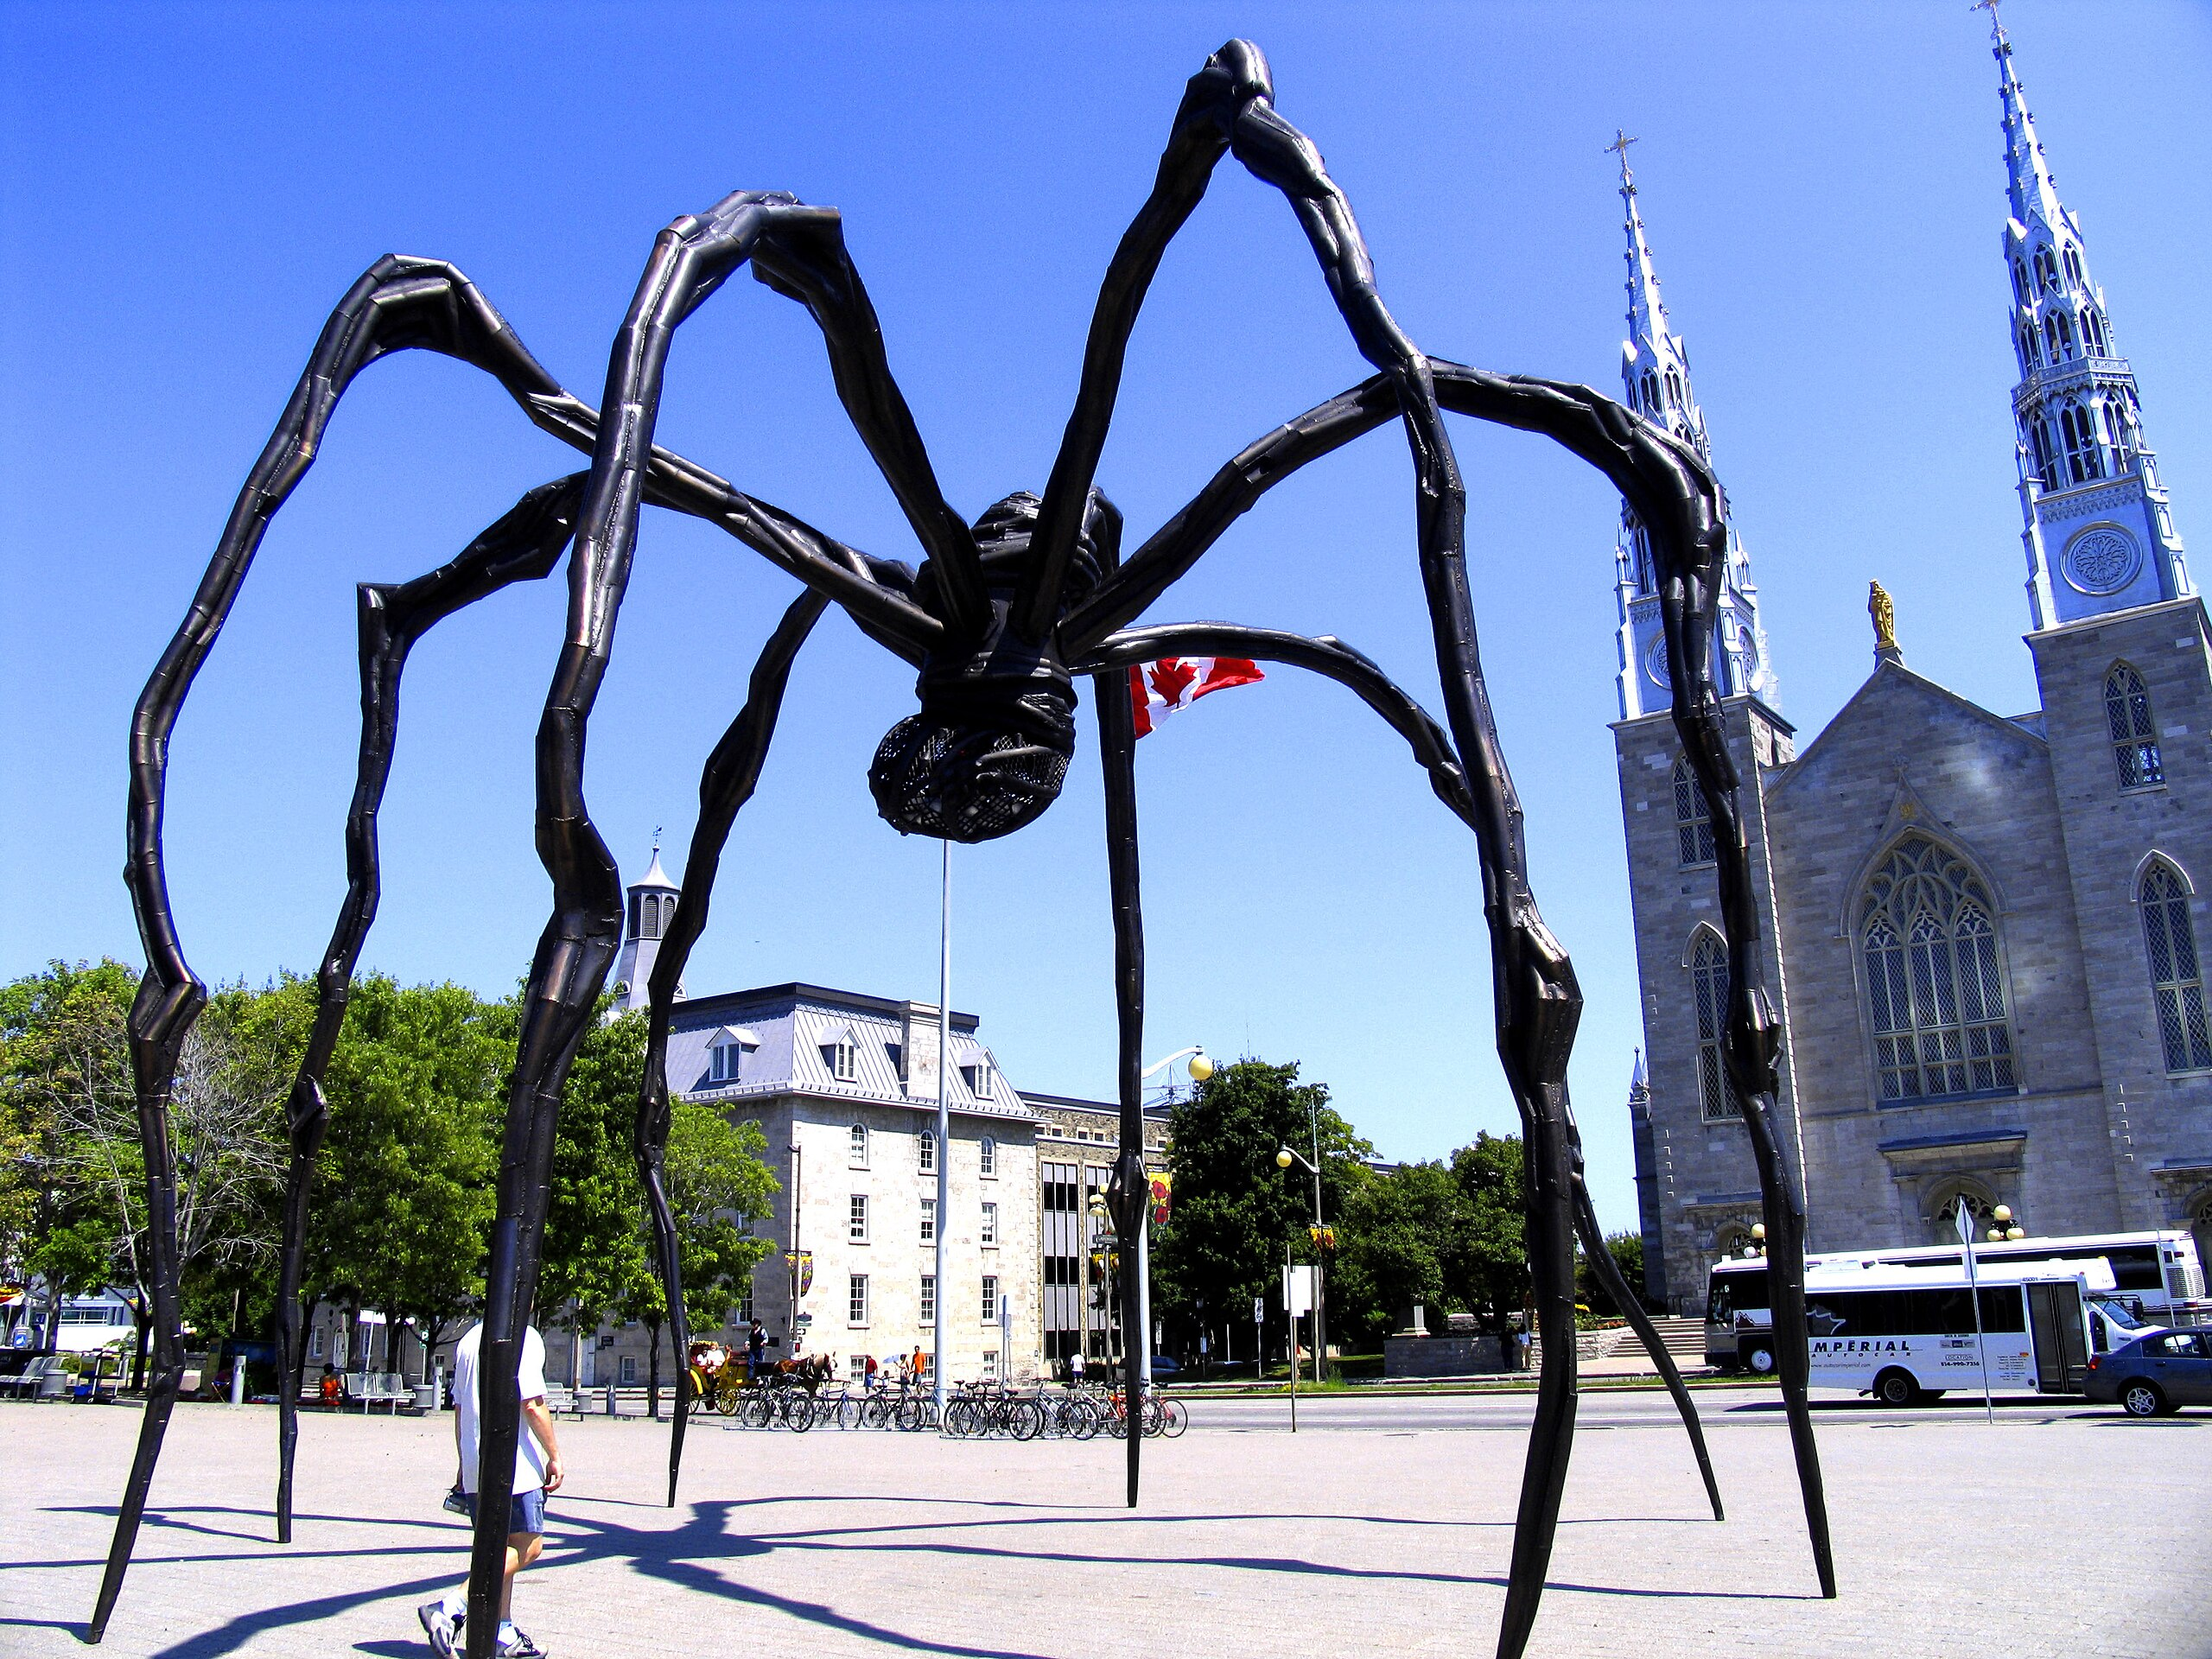
\includegraphics[width=0.98\linewidth]{img/maman.jpg}
    \end{subfigure}
    \begin{subfigure}{0.23\textwidth}
        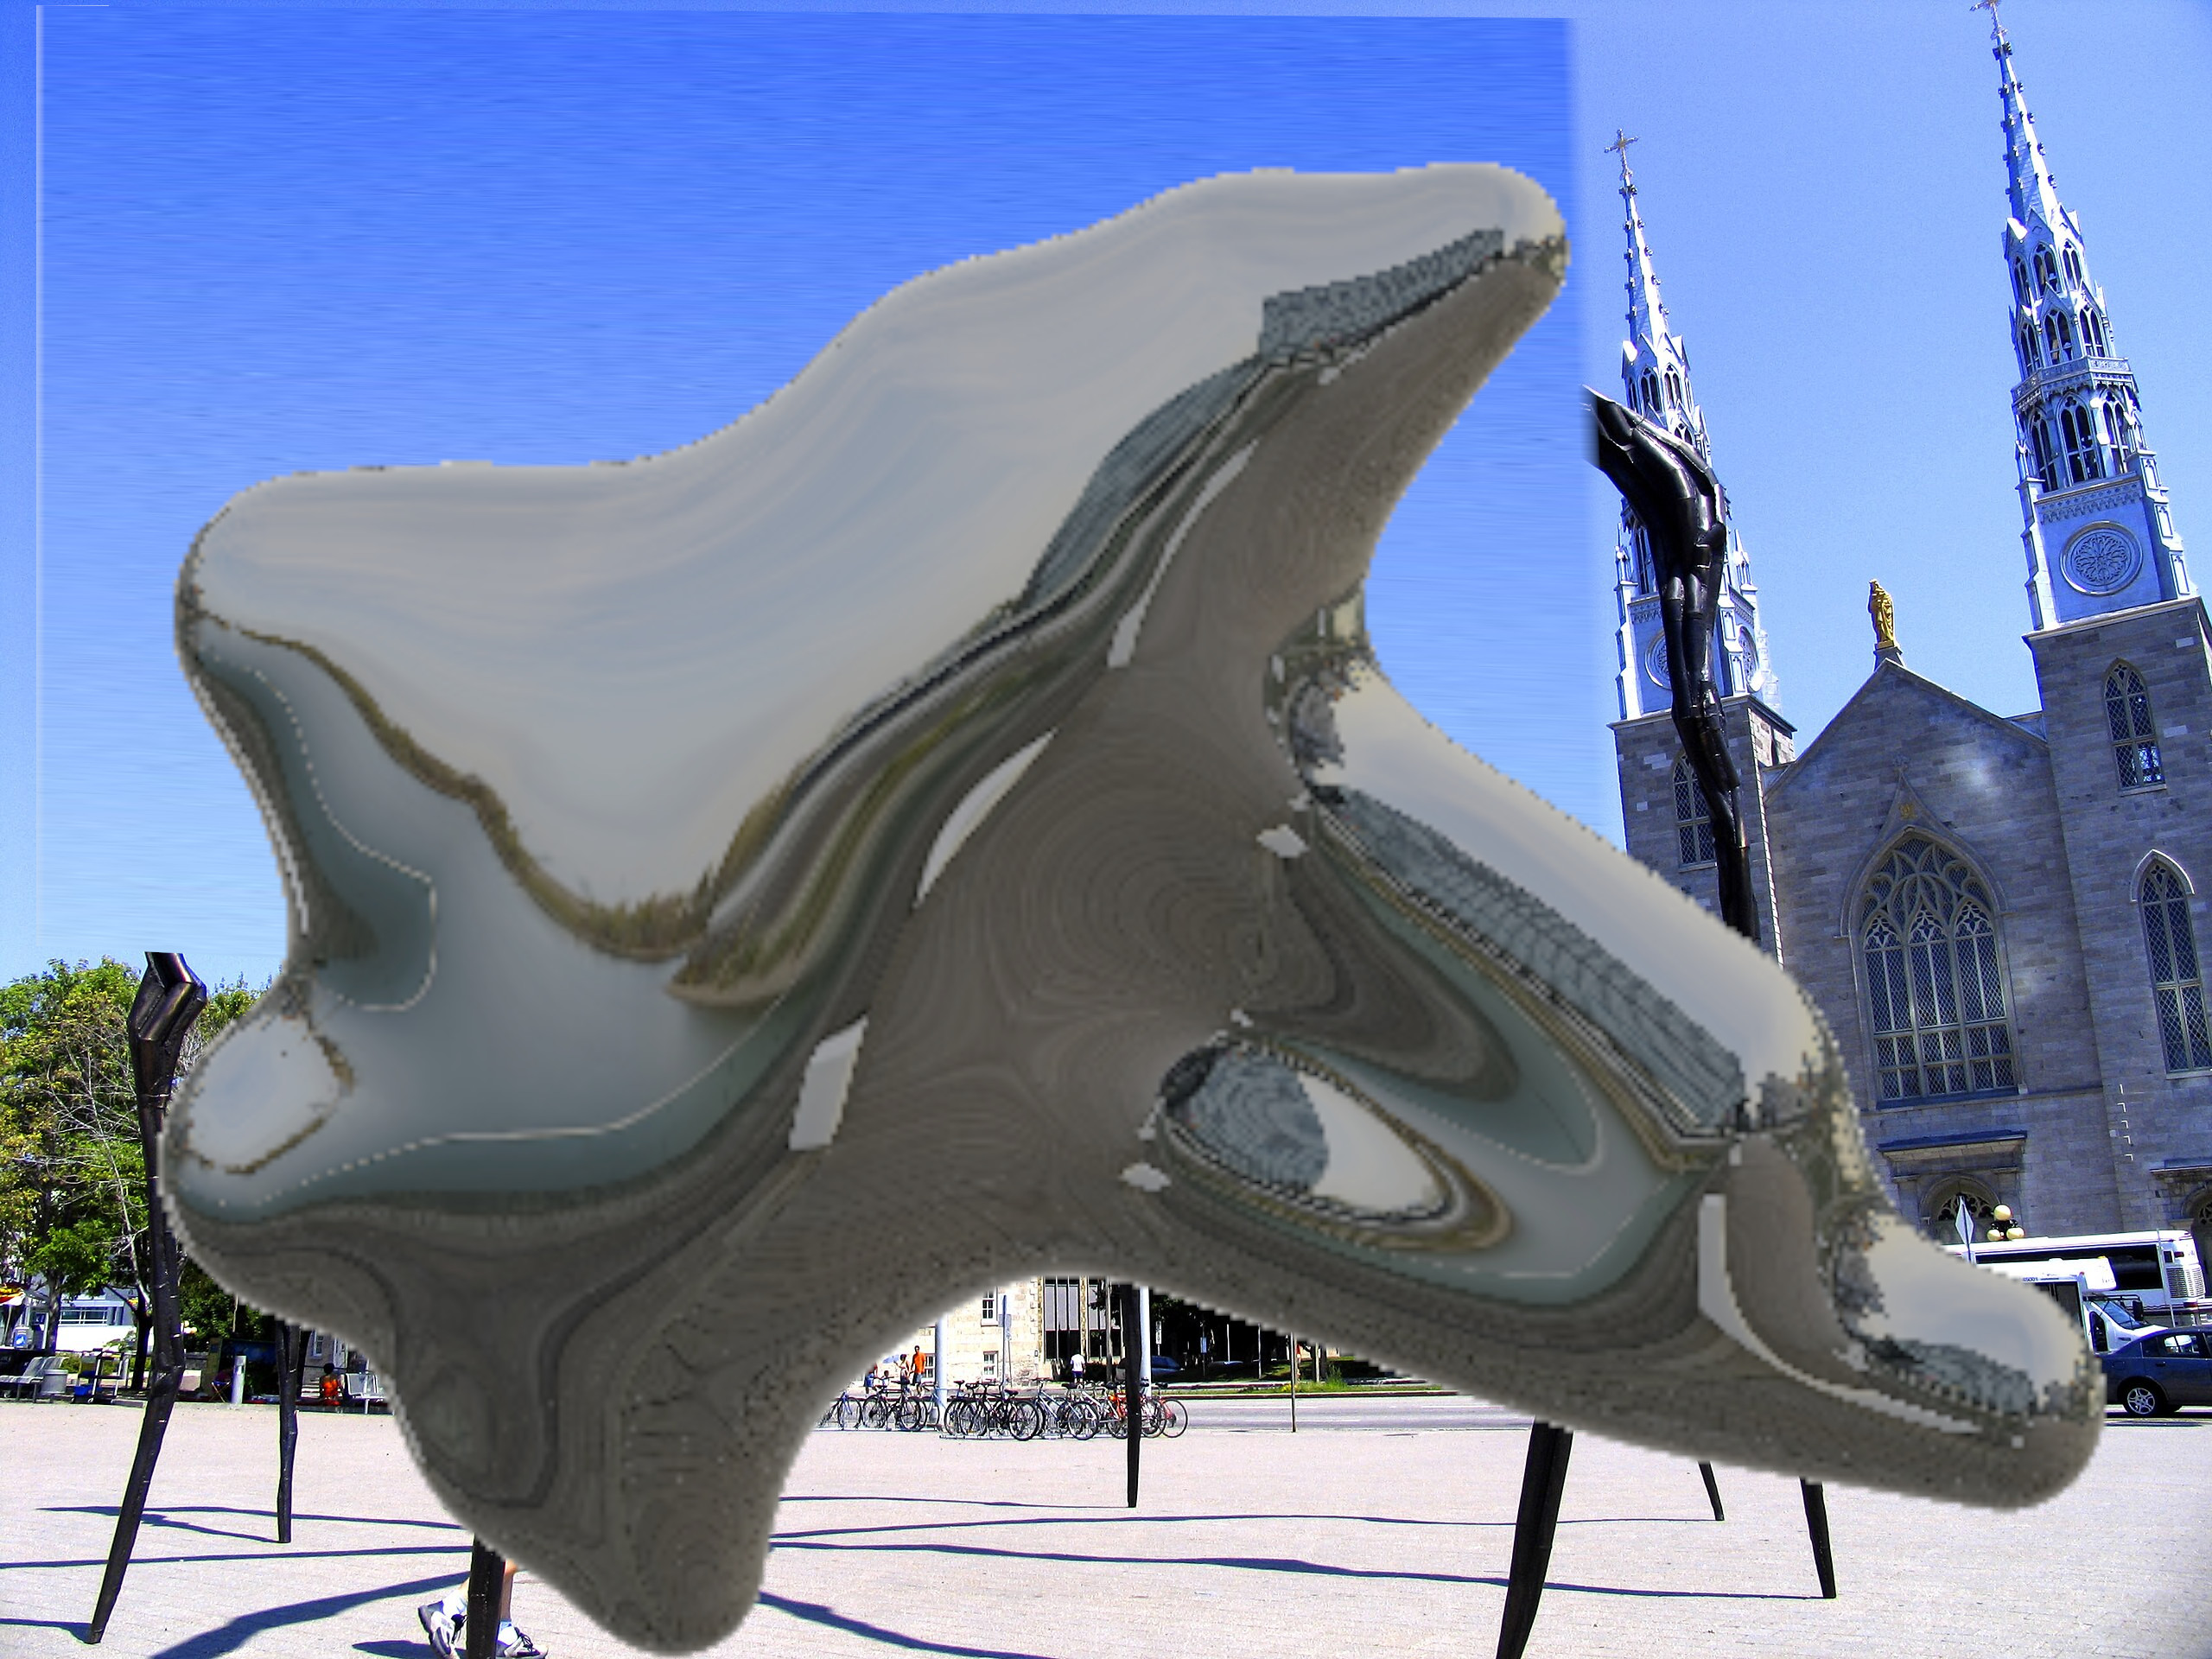
\includegraphics[width=0.98\linewidth]{img/maman-bean.jpg}
    \end{subfigure}
    \\
    \begin{subfigure}{0.23\textwidth}
        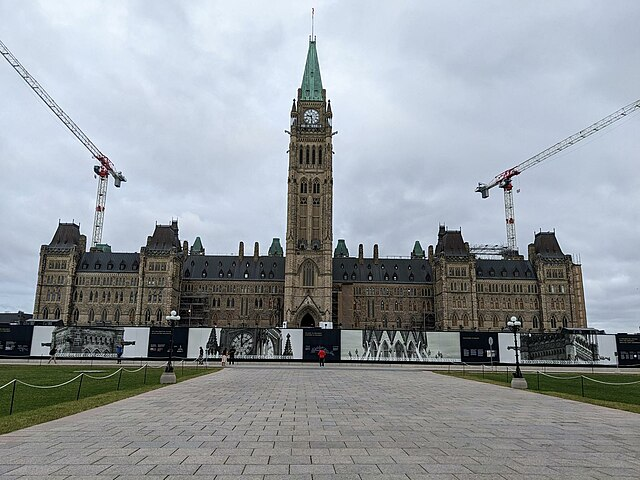
\includegraphics[width=0.98\linewidth]{img/Parliament_of_Canada_Building.jpg}
    \end{subfigure}
    \begin{subfigure}{0.23\textwidth}
        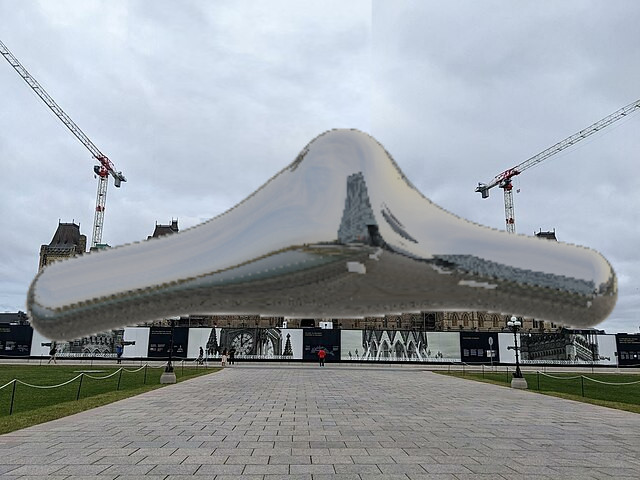
\includegraphics[width=0.98\linewidth]{img/parliament-bean-replacement.jpg}
    \end{subfigure}
    \caption{Beaned Ottawa landmarks: \emph{Maman} by Louise Bourgeois (photo by John Talbot, CC BY 2.0), and the Parliament buildings.}
    \label{fig:ottawa}
\end{figure}

\subsection{Novel Inputs}

Figure~\ref{fig:landmarks} shows yet more examples of Canadian and world landmarks replaced by beans. The beans effectively retain the form and character of the originals. The BN Tower maintains the same erect stature as the CN Tower (Figure~\ref{fig:landmarks}, first row.) In Pisa, tourists can still pose and hold up the Beaning Tower the same way they would have held up the Leaning Tower (Figure~\ref{fig:landmarks}, second row.) We believe this tight integration with the environment is sure to increase bean acceptance and tourism.


\section{Conclusion}
\label{section:conclusion}

Having established the economic advantage of replacing tired monuments with bean sculptures, we have presented an algorithm for designing bean sculptures on the basis of these existing landmarks: We establish a model of bean-space by creating smooth-unioned ensembles of simple beans, each parametrized by a quadratic B\'ezier curve. The parameters of the hyper-bean are then optimized to achieve the best fit to a given landmark. We apply our model to some example landmarks and we find good results, even with a relatively low-dimensional bean space. These results can be improved upon simply by increasing the number of parameters used in defining the hyper-bean; the cost of computing time for this should be small compared to the cost of hiring actual people to design beans. 


\begin{figure}[H]
    \begin{subfigure}{0.23\textwidth}
        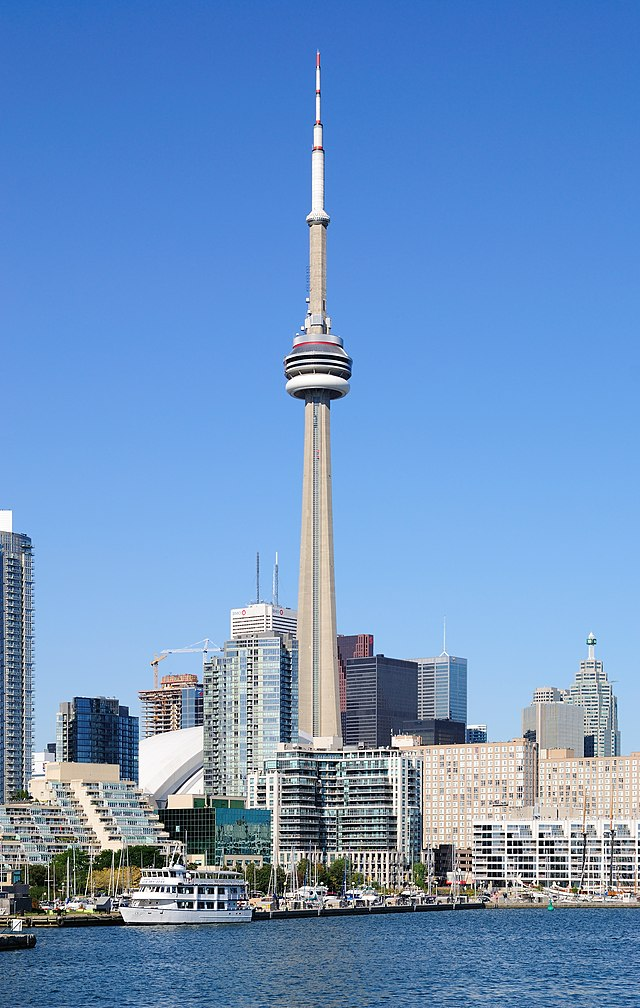
\includegraphics[width=0.98\linewidth]{img/Toronto_-_ON_-_Toronto_Harbourfront7.jpg}
    \end{subfigure}
    \begin{subfigure}{0.23\textwidth}
        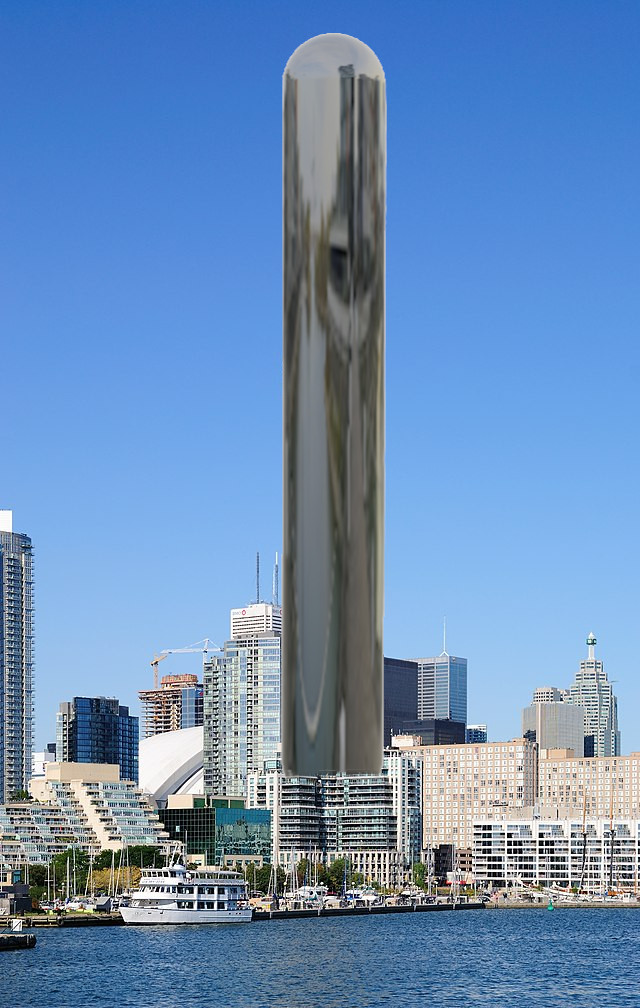
\includegraphics[width=0.98\linewidth]{img/cn-bean-waterfront.jpg}
    \end{subfigure}
    \\
    \begin{subfigure}{0.23\textwidth}
        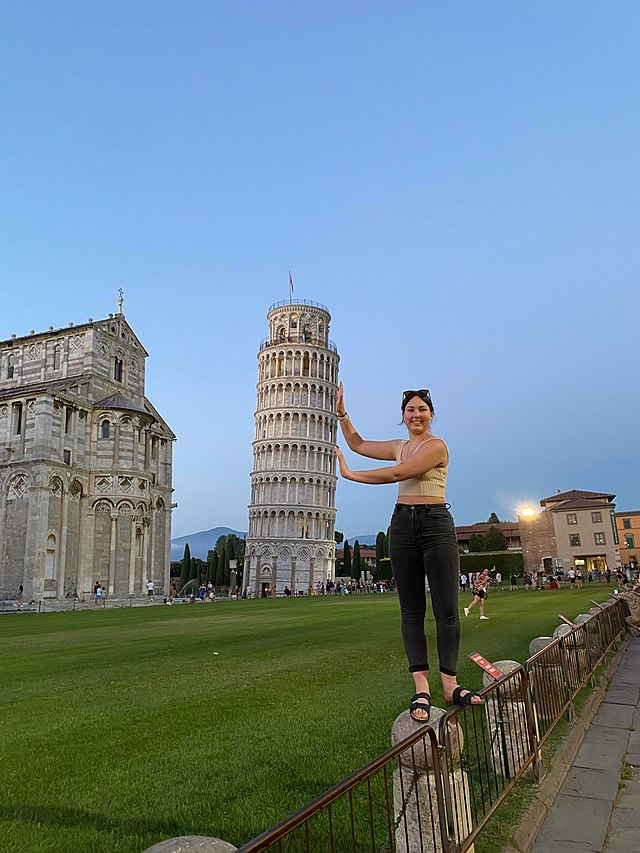
\includegraphics[width=0.98\linewidth]{img/pisa-tourist.jpg}
    \end{subfigure}
    \begin{subfigure}{0.23\textwidth}
        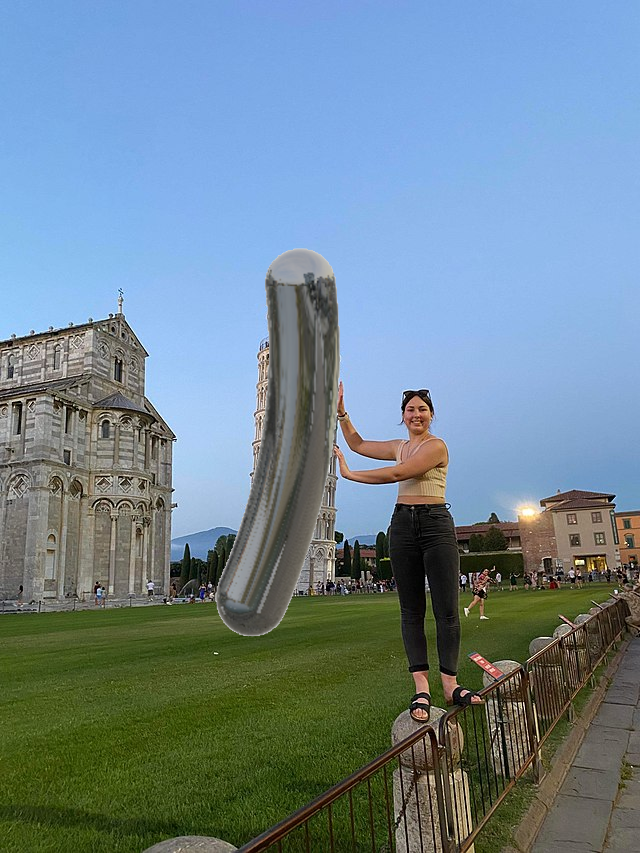
\includegraphics[width=0.98\linewidth]{img/pisa-tourist-bean.png}
    \end{subfigure}
    \\
    \begin{subfigure}{0.23\textwidth}
        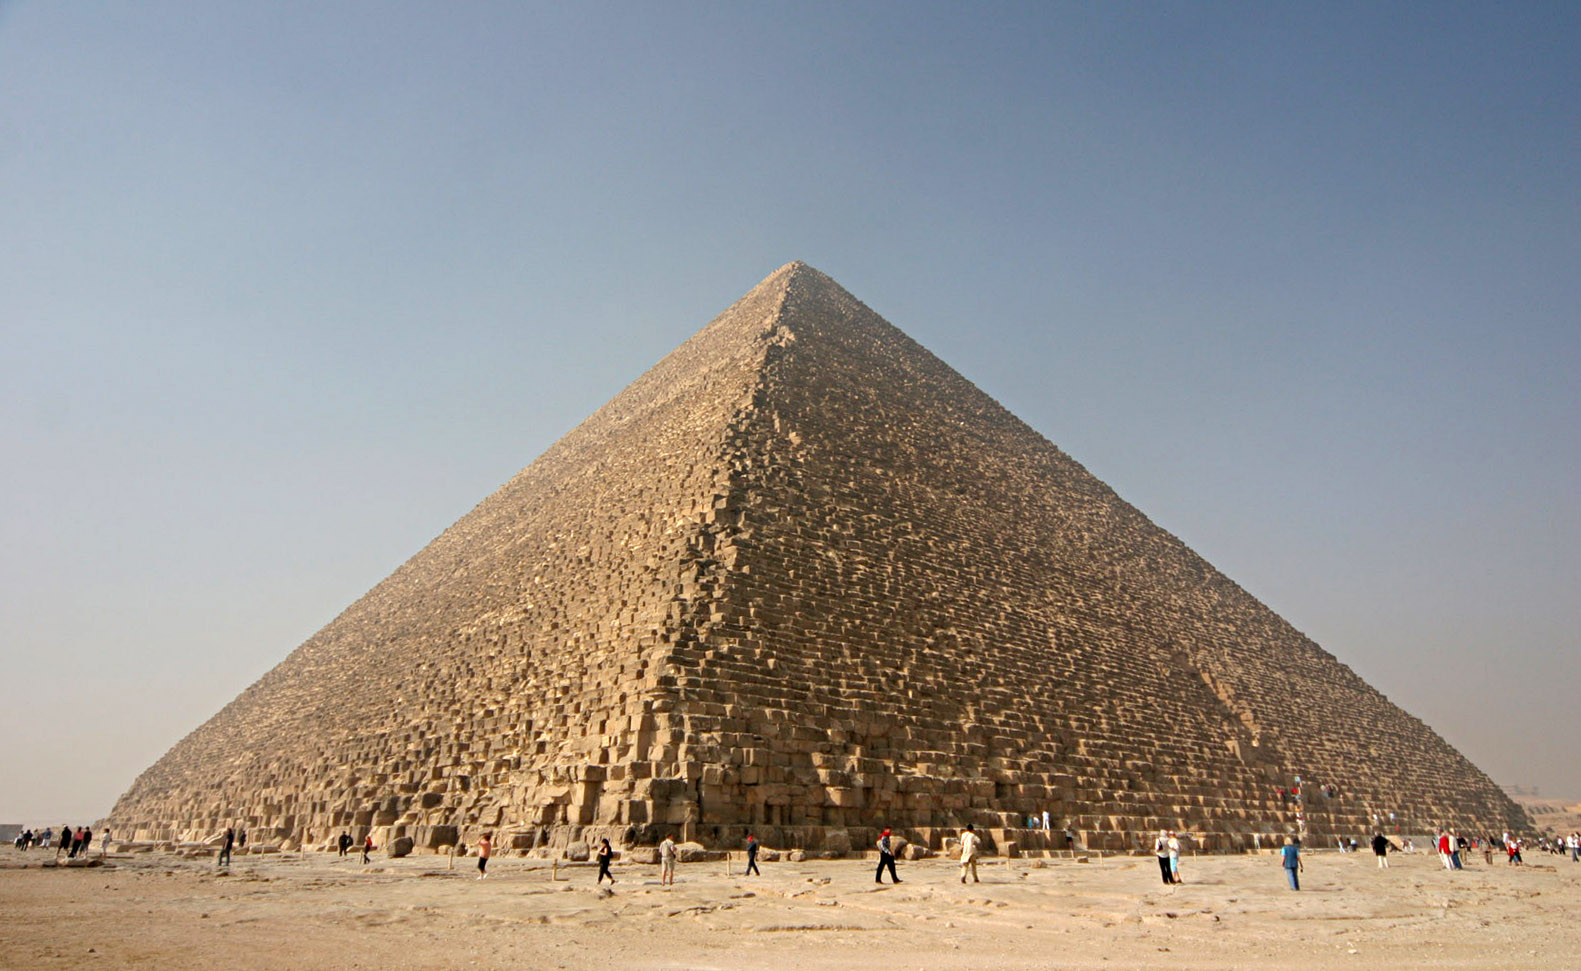
\includegraphics[width=0.98\linewidth]{img/Kheops-Pyramid.jpg}
    \end{subfigure}
    \begin{subfigure}{0.23\textwidth}
        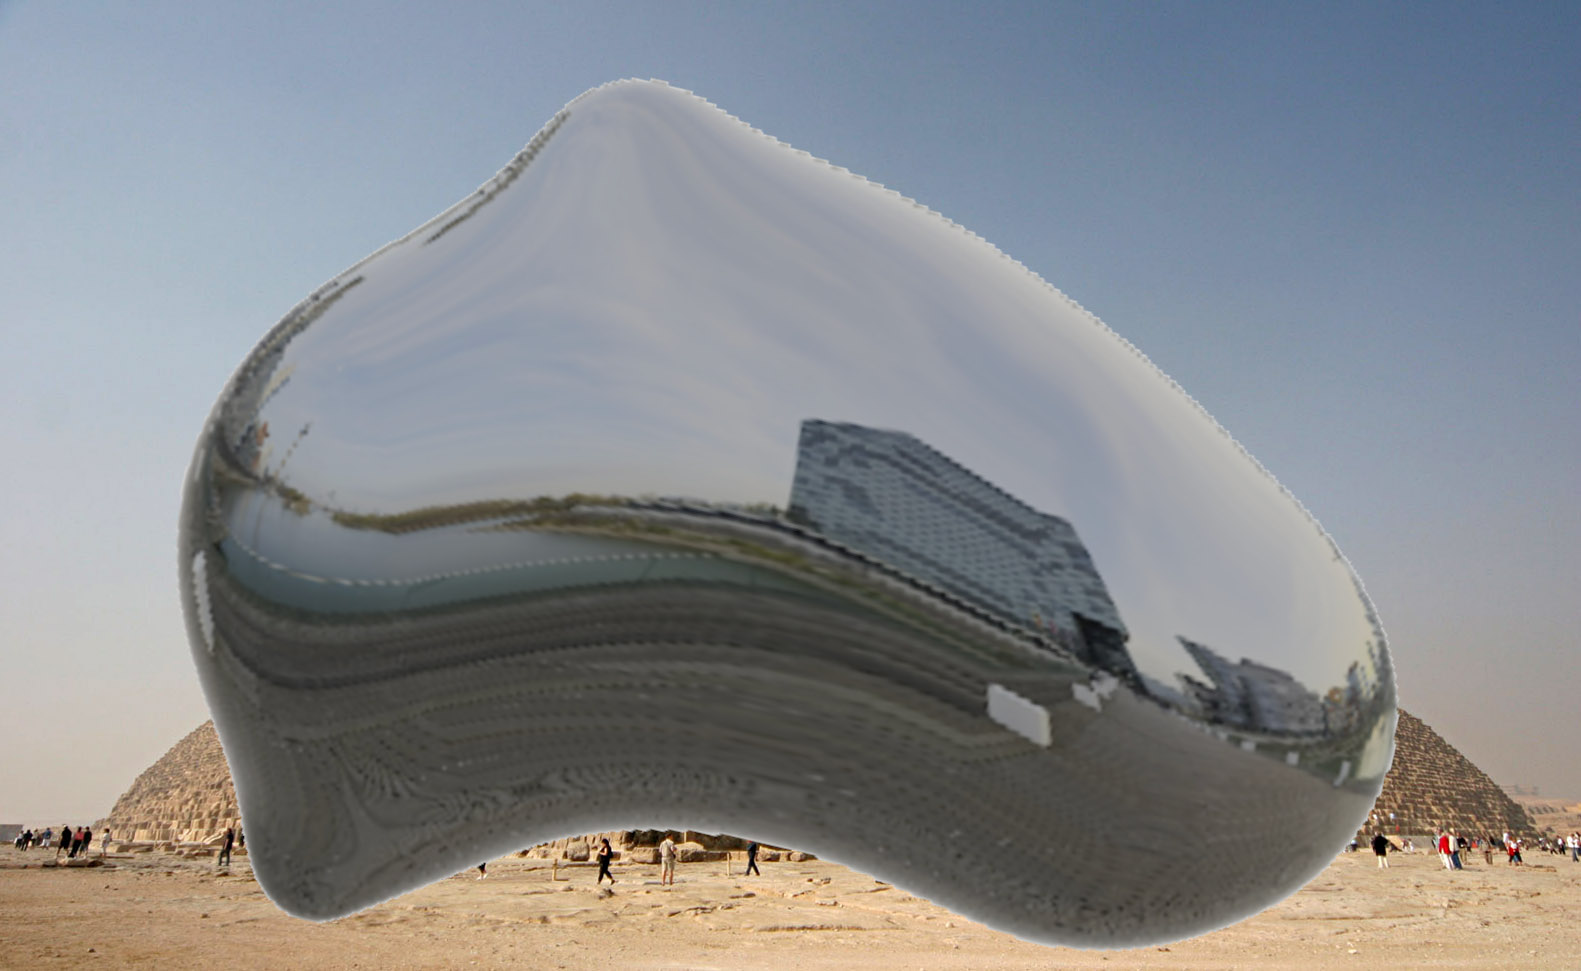
\includegraphics[width=0.98\linewidth]{img/pyramid-bean.jpg}
    \end{subfigure}
    \\
    \begin{subfigure}{0.23\textwidth}
        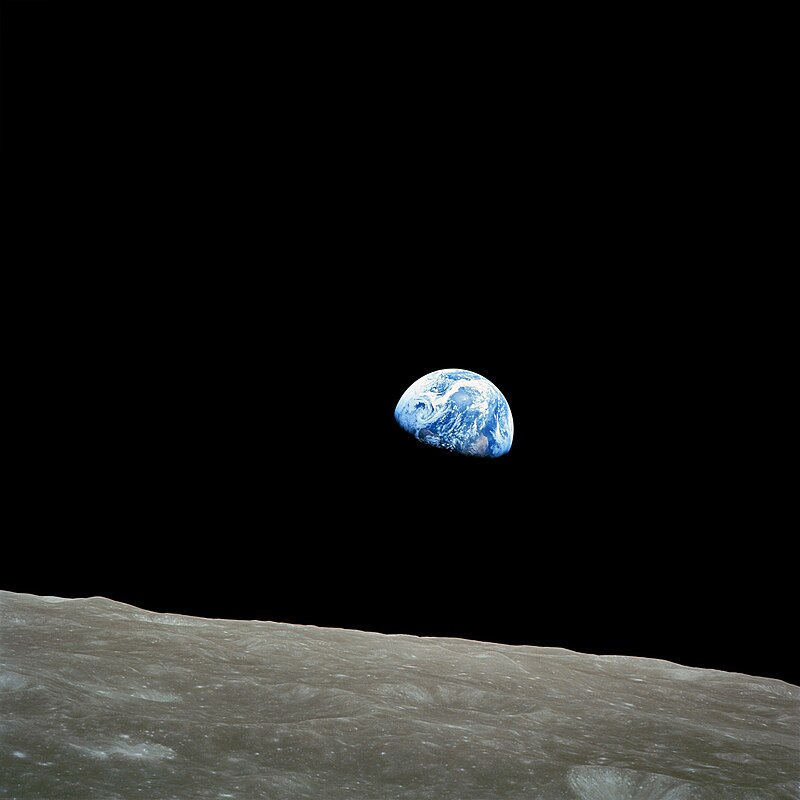
\includegraphics[width=0.98\linewidth]{img/earthrise.jpg}
    \end{subfigure}
    \begin{subfigure}{0.23\textwidth}
        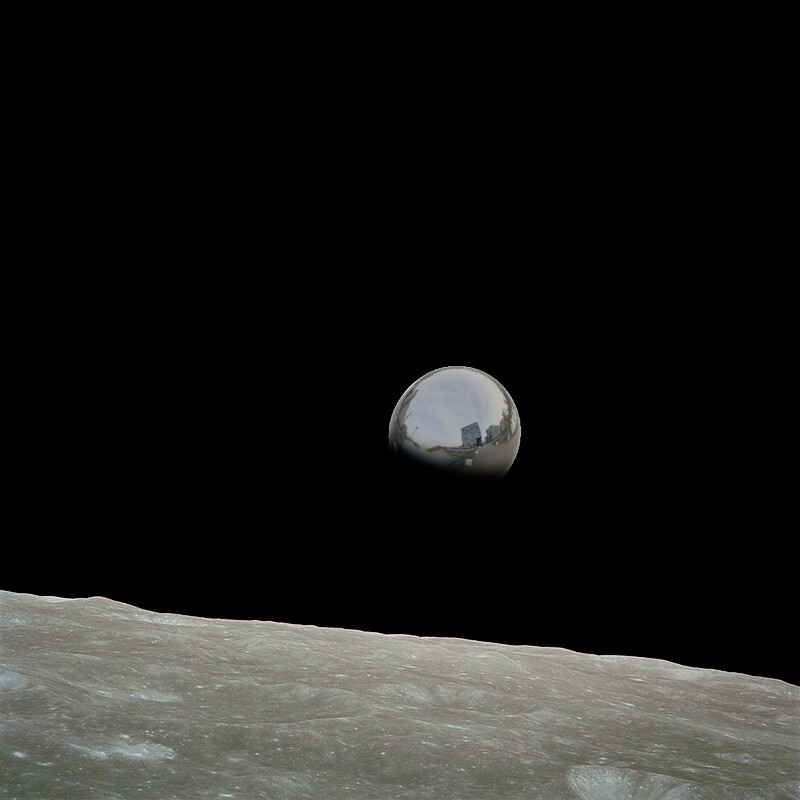
\includegraphics[width=0.98\linewidth]{img/bean-earth.jpg}
    \end{subfigure}
    \caption{Improved world landmarks: the CN Tower (photo by Wikimedia Commons user Wladyslaw, CC BY-SA 3.0), the Leaning Tower of Pisa (photo by Wikimedia Commons user U3207458, CC BY-SA 4.0), the Great Pyramid of Giza (photo by Wikimedia Commons user Nina, CC BY 2.5), and the Earth (photo by NASA/Bill Anders)}
    \label{fig:landmarks}
\end{figure}



We also envision extending this model to create beans for other purposes, beyond public art installations and/or upgrades to existing infrastructure and landmarks. For example, there may be a market for smaller personal beans, or even custom beans based on objects with some personal significance or sentimental value. 

But let not the motivation for the proliferation of beans be only capitalistic. As a society, we need beans. Their reflective surface inspires us to take a close look at ourselves. Their smooth contours and cold surfaces are soothing, a much needed balm in the feverish times of this 21st century. In the warped surface of a bean, one sees one's surroundings distorted, and one is inspired to see the world from a new perspective. Our world of right angles and matte surfaces has gotten us this far, but to progress further as a species, it is crucial that we embrace a radically different attitude in the decoration of our public and private spaces. The model we have presented in this work will without a doubt be an important tool in this effort of beanification. 




\section*{Acknowledgements}
The authors thank the R(izzness)atJOPT group chat for their comments throughout the preparation of this manuscript. MB thanks Anna Xu and Lyn Vakulenko for useful discussions. DP thanks the City of Chicago for the existence of such delights as the Bean and the Rat Hole.


\bibliographystyle{plainurl}
\bibliography{main}

\end{document}
%
% ****** End of file apssamp.tex ******
